\documentclass[conference]{IEEEtran}
\IEEEoverridecommandlockouts

\usepackage[utf8]{inputenc}
\usepackage[T1]{fontenc}
\usepackage{cite}
\usepackage{amsmath,amssymb,amsfonts}
\usepackage{graphicx}
\usepackage{textcomp}
\usepackage{xcolor}
\usepackage{url}

\def\BibTeX{{\rm B\kern-.05em{\sc i\kern-.025em b}\kern-.08em
    T\kern-.1667em\lower.7ex\hbox{E}\kern-.125emX}}


\begin{document}

\title{Road Pitch Estimation and Sensor Fusion in CARLA Using Semantic Camera Measurements}

\author{
\IEEEauthorblockN{Rüzgar Batı Okay}
\IEEEauthorblockA{
Department of Electrical and Electronics Engineering\\
Marmara University\\
Istanbul, Türkiye\\
ruzgarbatiokay25072003@gmail.com
}
\and
\IEEEauthorblockN{Alperen Tufan Pelit}
\IEEEauthorblockA{
Department of Electrical and Electronics Engineering\\
Marmara University\\
Istanbul, Türkiye\\
pelitalperentufan@gmail.com
}
}

\maketitle


\begin{abstract}
Accurate road pitch estimation is important for autonomous vehicle state estimation and longitudinal control. This project investigates a CARLA 0.9.16-based pitch estimation pipeline using simulated inertial, camera, and global navigation satellite system measurements. The original camera measurement approach based on geometric horizon or vanishing-point extraction was replaced with a supervised MobileNet-based regression model trained on CARLA semantic road and road-line masks. Since this replacement provides pitch directly as the camera measurement, the implemented pitch-only fusion model reduces to a linear Kalman Filter. In this structure, the inertial measurement unit gyroscope provides the prediction input, while the camera model provides the measurement correction. CARLA vehicle pitch and waypoint road pitch are used as reference signals. Experimental results show that the camera and Kalman Filter estimates closely follow the reference pitch profile under the controlled simulation route, while the GNSS-derived pitch estimate becomes unavailable or unreliable when vehicle displacement is insufficient.
\end{abstract}

\begin{IEEEkeywords}
CARLA, pitch estimation, semantic segmentation, MobileNet, IMU, GNSS, Kalman Filter, sensor fusion.
\end{IEEEkeywords}

% ============================================================
% Main text
% ============================================================

\section{Introduction}
Road pitch and road-parameter estimation are relevant state-estimation problems for autonomous vehicles because road geometry affects perception, localization, longitudinal dynamics, and control decisions. Previous work has investigated iterative road-parameter estimation using monocular camera measurements and Kalman-filter-related estimation methods \cite{ustunel2023iterative}. In this project, the same general road-pitch estimation problem is recreated in a CARLA-based simulation environment \cite{dosovitskiy2017carla}.

The initial project proposal considered a sensor-fusion structure in which inertial measurement unit (IMU) data was used for prediction and camera-based pitch measurements were used for correction. The original camera measurement was planned to be obtained through geometric horizon or vanishing-point extraction from lane markings. In that case, the camera geometry would introduce nonlinear measurement relations. However, this method was unreliable in the selected simulation setup due to unstable visual line extraction. Therefore, the camera measurement block was replaced with a supervised learning model trained on CARLA semantic segmentation masks.

After this change, the camera system provides pitch directly as a scalar measurement. Therefore, the implemented pitch-only fusion model becomes linear and is implemented as a standard Kalman Filter (KF), while preserving the original prediction-correction sensor-fusion architecture. The nonlinear mapping from image geometry to pitch is handled by the MobileNet regression model before the filtering stage.

The main contributions of the implemented system are:
\begin{itemize}
    \item collecting a CARLA dataset of semantic road and road-line masks with pitch labels,
    \item training a lightweight MobileNet regression model to estimate pitch from semantic road geometry,
    \item logging synchronized camera, IMU, GNSS, vehicle ground truth, and waypoint reference data,
    \item implementing IMU-prediction and camera-correction based KF fusion,
    \item comparing camera-based, GNSS-derived, and KF pitch estimates against CARLA reference signals.
\end{itemize}



\section{Simulation Environment}

\subsection{CARLA Setup}
Experiments were performed in CARLA 0.9.16 using the \textit{Town05} map, which contains curved roads, ramps, and traffic-control elements suitable for observing pitch changes. CARLA was selected because it provides a controllable autonomous driving simulation environment with vehicle actors, sensor actors, traffic behavior, and access to ground-truth vehicle states \cite{dosovitskiy2017carla}. A Tesla Model 3 vehicle actor from the CARLA blueprint library was used throughout the experiments. Vehicle type selection was not a primary variable in this study. The vehicle was driven using CARLA autopilot in synchronous simulation mode with a fixed time step of 0.05 s.

\subsection{Software Environment}
The implementation was developed in Python 3.11 \cite{pythonSoftware}. The CARLA client interface used the Python 3.11 wheel compatible with CARLA 0.9.16, and the simulator was controlled through the CARLA Python API \cite{carlaPythonAPI}. The machine-learning pipeline was implemented using PyTorch \cite{paszke2019pytorch}, and CUDA acceleration was used during model training. The trained MobileNetV3-small regression model was then loaded by the main CARLA script for online camera-based pitch estimation \cite{howard2019mobilenetv3}.

\subsection{Reference Pitch Signals}
Two reference pitch signals were logged during the experiment. The first reference is the true vehicle pitch obtained directly from the CARLA vehicle transform. The second reference is the waypoint road pitch obtained from the CARLA map waypoint at the current vehicle position. The vehicle pitch represents the simulated body orientation, while the waypoint pitch represents the road-grade reference.

\section{Sensor Measurement Generation}

\subsection{Semantic Camera}
A CARLA semantic segmentation camera was mounted at the front of the vehicle. The image resolution was set to 1280$\times$720 pixels with a horizontal field of view of 90 degrees and a sensor period of 0.05 s. The CARLA sensor framework was used to configure the semantic camera, IMU, and GNSS sensors \cite{carlaSensors}. Instead of using raw RGB images, only semantic classes corresponding to road and road-line markings were retained.

\subsection{Inertial Measurement Unit}
The IMU was mounted on the vehicle and used to log acceleration, angular velocity, and compass values. For the implemented filter, only the gyroscope pitch-rate component is used as the prediction input. The accelerometer channels were logged for completeness but were not used as a separate pitch measurement because the proposed fusion structure uses the camera as the correction source.

\subsection{Global Navigation Satellite System}
The global navigation satellite system (GNSS) sensor was used as an additional baseline. GNSS-derived pitch was computed from altitude change over horizontal displacement between consecutive valid GNSS samples. Because this method depends on vehicle motion, it may become unavailable when the vehicle is stationary or moving too slowly.

\section{Camera-Based Pitch Estimation}

\subsection{Semantic Road and Road-Line Masking}
The semantic camera output was converted into a three-channel mask image. The first channel represents the road region, the second channel represents road-line markings, and the third channel represents the combined road and road-line mask. This representation removes unrelated objects such as buildings, poles, vehicles, and sky, forcing the model to estimate pitch from road geometry.

\begin{figure}[t]
    \centering
    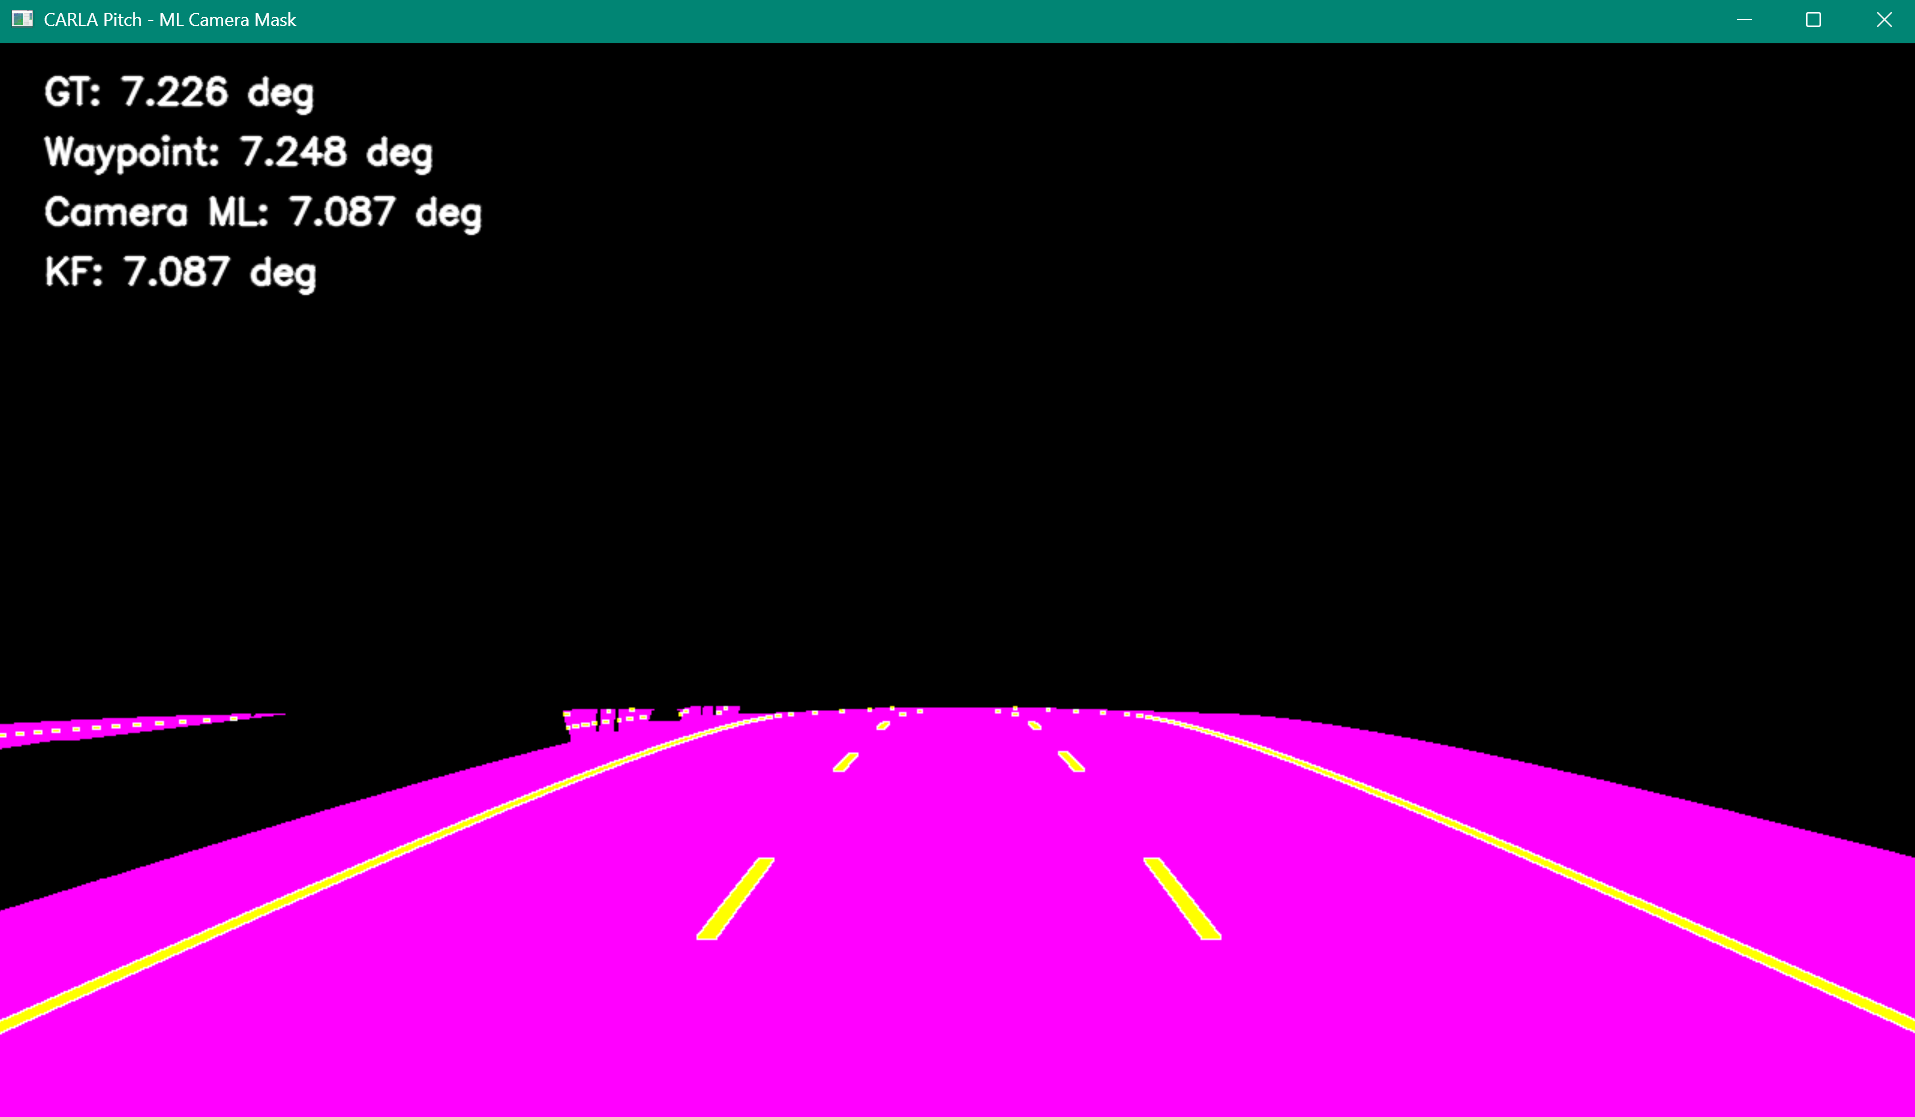
\includegraphics[width=\linewidth]{figures/semantic_mask_example.png}
    \caption{Example semantic road and road-line mask used as input to the MobileNet pitch regression model. Road pixels are shown in magenta and road-line pixels are shown in yellow.}
    \label{fig:semantic_mask}
\end{figure}

\subsection{Dataset Collection}
A dataset was collected by driving the vehicle in the selected Town05 route and saving semantic road and road-line masks together with pitch labels. The dataset was split into training and validation subsets using an 80/20 split. The training label used for the current model was the true vehicle pitch obtained from CARLA. The waypoint pitch was also stored for evaluation and comparison.

\subsection{MobileNet Regression Model}
A MobileNetV3-small architecture was used as a lightweight convolutional regression model. MobileNetV3 was selected because it is designed as an efficient convolutional network family for low-resource inference scenarios \cite{howard2019mobilenetv3}. The original classification head was replaced with a single-output fully connected layer that predicts pitch in degrees. The input to the network is the semantic road and road-line mask resized to 224$\times$224 pixels.

The learned camera measurement can be written as
\begin{equation}
    z^{\mathrm{cam}}_k = f_{\theta}(I^{\mathrm{mask}}_k),
    \label{eq:camera_model}
\end{equation}
where $I^{\mathrm{mask}}_k$ is the road and road-line mask at time step $k$, $f_{\theta}$ is the trained MobileNet regression model, and $z^{\mathrm{cam}}_k$ is the estimated pitch angle.

\subsection{Training Procedure}
The MobileNetV3-small regression model was trained using supervised learning on the collected semantic road and road-line mask dataset. The implementation was developed in Python 3.11 and trained using PyTorch \cite{pythonSoftware,paszke2019pytorch}. The dataset was divided into training and validation subsets using an 80/20 split. Input images were resized to 224$\times$224 pixels before being passed to the network.

The target output of the network was the true vehicle pitch obtained directly from CARLA ground-truth vehicle orientation. The model was trained for 30 epochs, and validation metrics were monitored after each epoch. The best-performing model checkpoint was saved and later used by the live CARLA pitch-estimation script.

\begin{figure}[t]
    \centering
    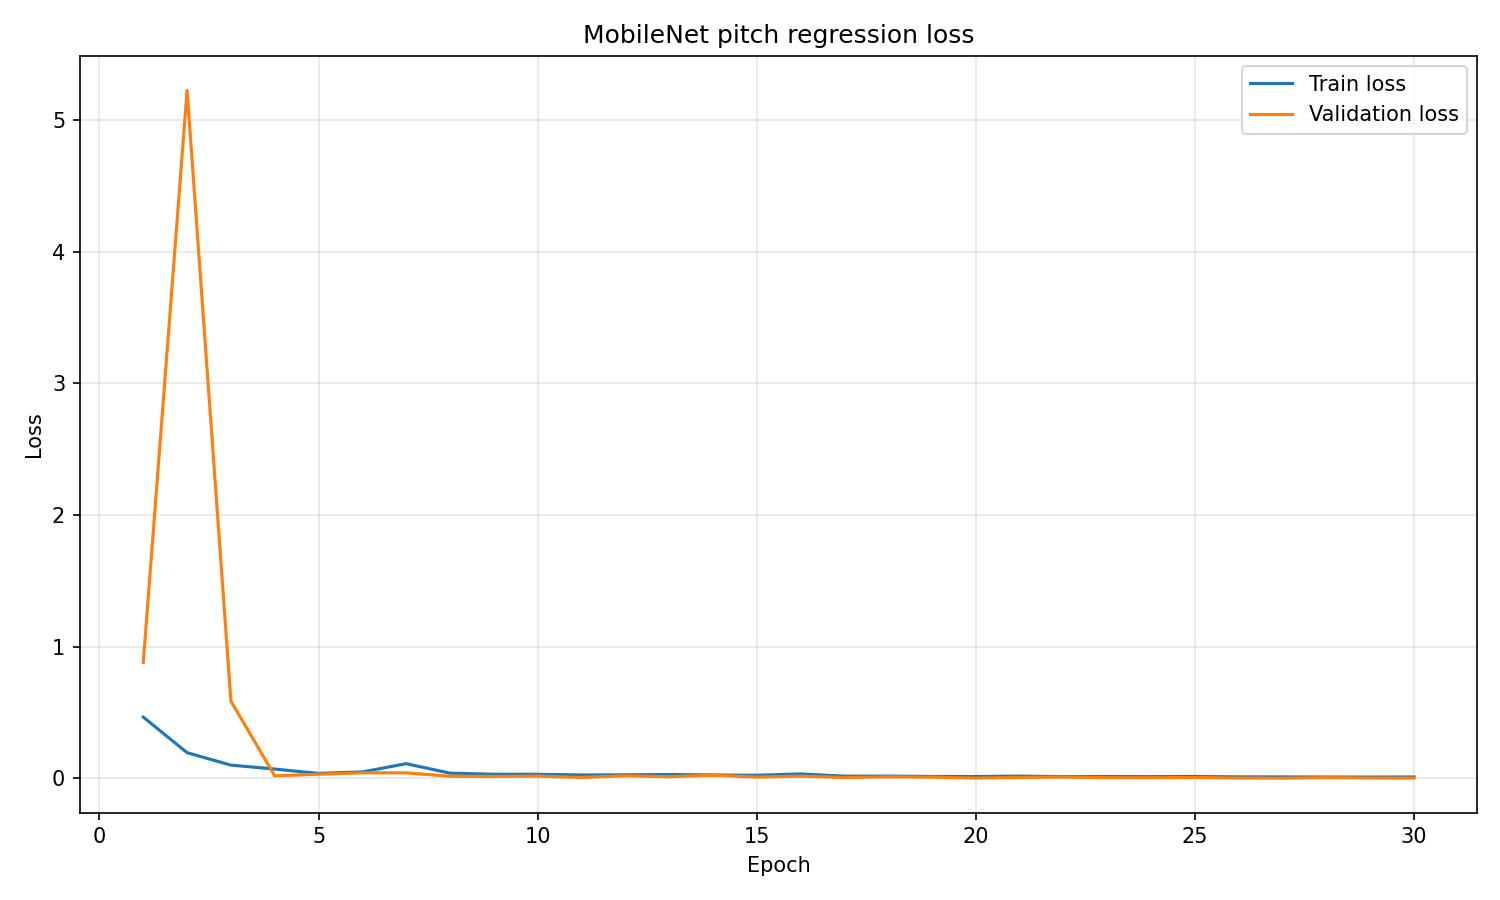
\includegraphics[width=\linewidth]{figures/loss_curve.png}
    \caption{Training and validation loss during MobileNet pitch regression.}
    \label{fig:loss_curve}
\end{figure}

The training and validation losses converged rapidly after the first few epochs, as shown in Fig. \ref{fig:loss_curve}. After convergence, both losses remained low with limited divergence, indicating that the model learned the pitch relationship from the semantic mask representation under the controlled CARLA route.

\begin{figure}[t]
    \centering
    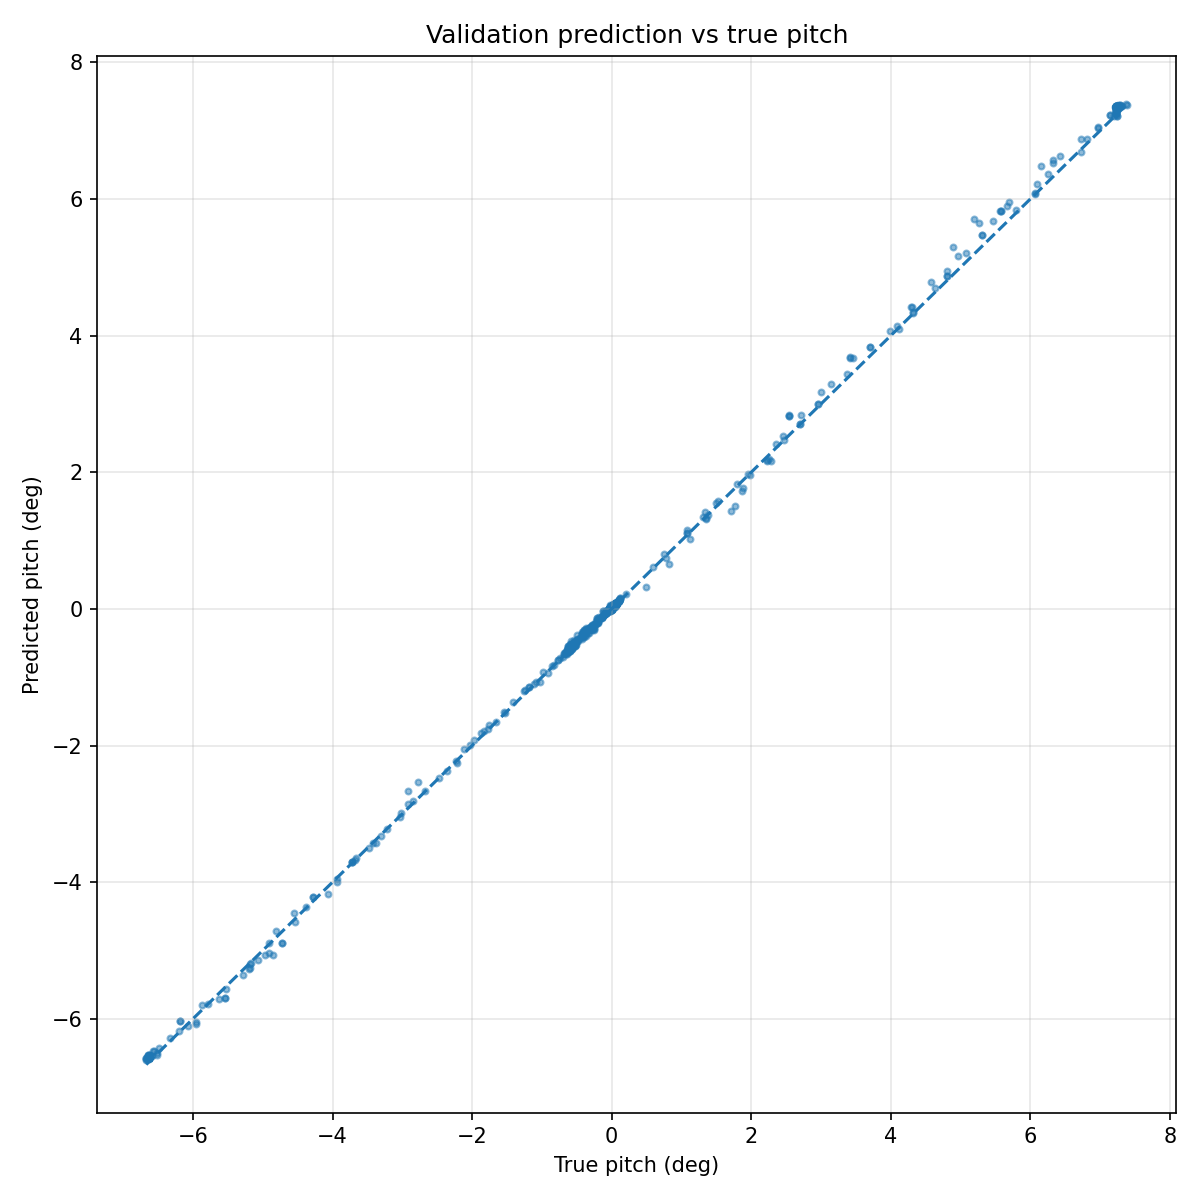
\includegraphics[width=\linewidth]{figures/val_prediction_vs_true_last.png}
    \caption{Validation predictions versus true pitch values for the trained MobileNet regression model.}
    \label{fig:val_scatter}
\end{figure}

Fig. \ref{fig:val_scatter} shows the predicted pitch values against the true validation labels. Most samples are close to the one-to-one prediction line, indicating that the trained model can estimate pitch accurately within the pitch range represented in the collected dataset.

\section{GNSS-Based Pitch Estimation}
The GNSS baseline estimates pitch using the altitude difference and horizontal distance between two consecutive valid GNSS measurements:
\begin{equation}
    \theta^{\mathrm{GNSS}}_k =
    \tan^{-1}\left(
    \frac{h_k - h_{k-1}}{d^{\mathrm{horizontal}}_k}
    \right),
    \label{eq:gnss_pitch}
\end{equation}
where $h_k$ is altitude and $d^{\mathrm{horizontal}}_k$ is the horizontal displacement between consecutive GNSS samples. A minimum horizontal displacement threshold was applied to avoid unstable pitch estimates when the vehicle was nearly stationary.

This limitation is important in traffic scenarios. For example, when the vehicle stops at a red light, the GNSS-derived pitch estimate becomes unavailable because there is insufficient horizontal displacement. In contrast, the camera model can still estimate pitch because it depends on the visible road geometry rather than vehicle motion.



\section{Kalman Filter Sensor Fusion Framework}

\subsection{Linear Pitch-State Formulation}
The original project proposal considered an EKF framework because the horizon or vanishing-point camera geometry was expected to be nonlinear. After replacing this geometric measurement stage with a direct MobileNet pitch regressor, the filter receives pitch directly as a measurement. Therefore, the implemented pitch-only fusion model reduces to a standard linear Kalman Filter.

The filter state is defined as
\begin{equation}
    x_k = \theta_k,
    \label{eq:kf_state}
\end{equation}
where $\theta_k$ is the pitch angle in degrees. The IMU gyroscope does not provide pitch directly; it provides pitch angular velocity. Therefore, the prediction step integrates the gyroscope pitch-rate measurement:
\begin{equation}
    \theta_{k|k-1} =
    \theta_{k-1|k-1} + \omega^{\mathrm{imu}}_{y,k}\Delta t,
    \label{eq:kf_prediction}
\end{equation}
where $\omega^{\mathrm{imu}}_{y,k}$ is the gyroscope pitch-rate measurement converted to degrees per second.

\subsection{Camera Measurement Update}
The camera measurement is the MobileNet pitch estimate:
\begin{equation}
    z_k = z^{\mathrm{cam}}_k = \theta_k + v_k.
    \label{eq:kf_measurement}
\end{equation}
Since the camera output is already an angle measurement, the scalar measurement matrix is $H=1$.

The prediction covariance update is
\begin{equation}
    P_{k|k-1} = P_{k-1|k-1} + Q,
    \label{eq:kf_cov_prediction}
\end{equation}
and the Kalman gain is
\begin{equation}
    K_k =
    \frac{P_{k|k-1}}{P_{k|k-1}+R}.
    \label{eq:kf_gain}
\end{equation}
The corrected pitch estimate is then
\begin{equation}
    \theta_{k|k} =
    \theta_{k|k-1} + K_k(z_k-\theta_{k|k-1}),
    \label{eq:kf_update}
\end{equation}
with covariance update
\begin{equation}
    P_{k|k} = (1-K_k)P_{k|k-1}.
    \label{eq:kf_cov_update}
\end{equation}

\subsection{Noise Parameters}
The process noise $Q$ controls the uncertainty added during IMU gyro integration, while the measurement noise $R$ controls the trust assigned to the camera pitch measurement. In the implemented run, both values were set to $Q=0.01$ and $R=0.01$. GNSS-derived pitch was not fused into the filter because it depends on horizontal displacement and may become unavailable when the vehicle is stationary.



\section{Experimental Results}

\subsection{Camera Pitch Estimation Results}
The trained camera model was evaluated during a live CARLA route using the same semantic mask generation pipeline. Fig. \ref{fig:camera_pitch} compares the camera pitch estimate with the true vehicle pitch and waypoint road pitch.

\begin{figure}[t]
    \centering
    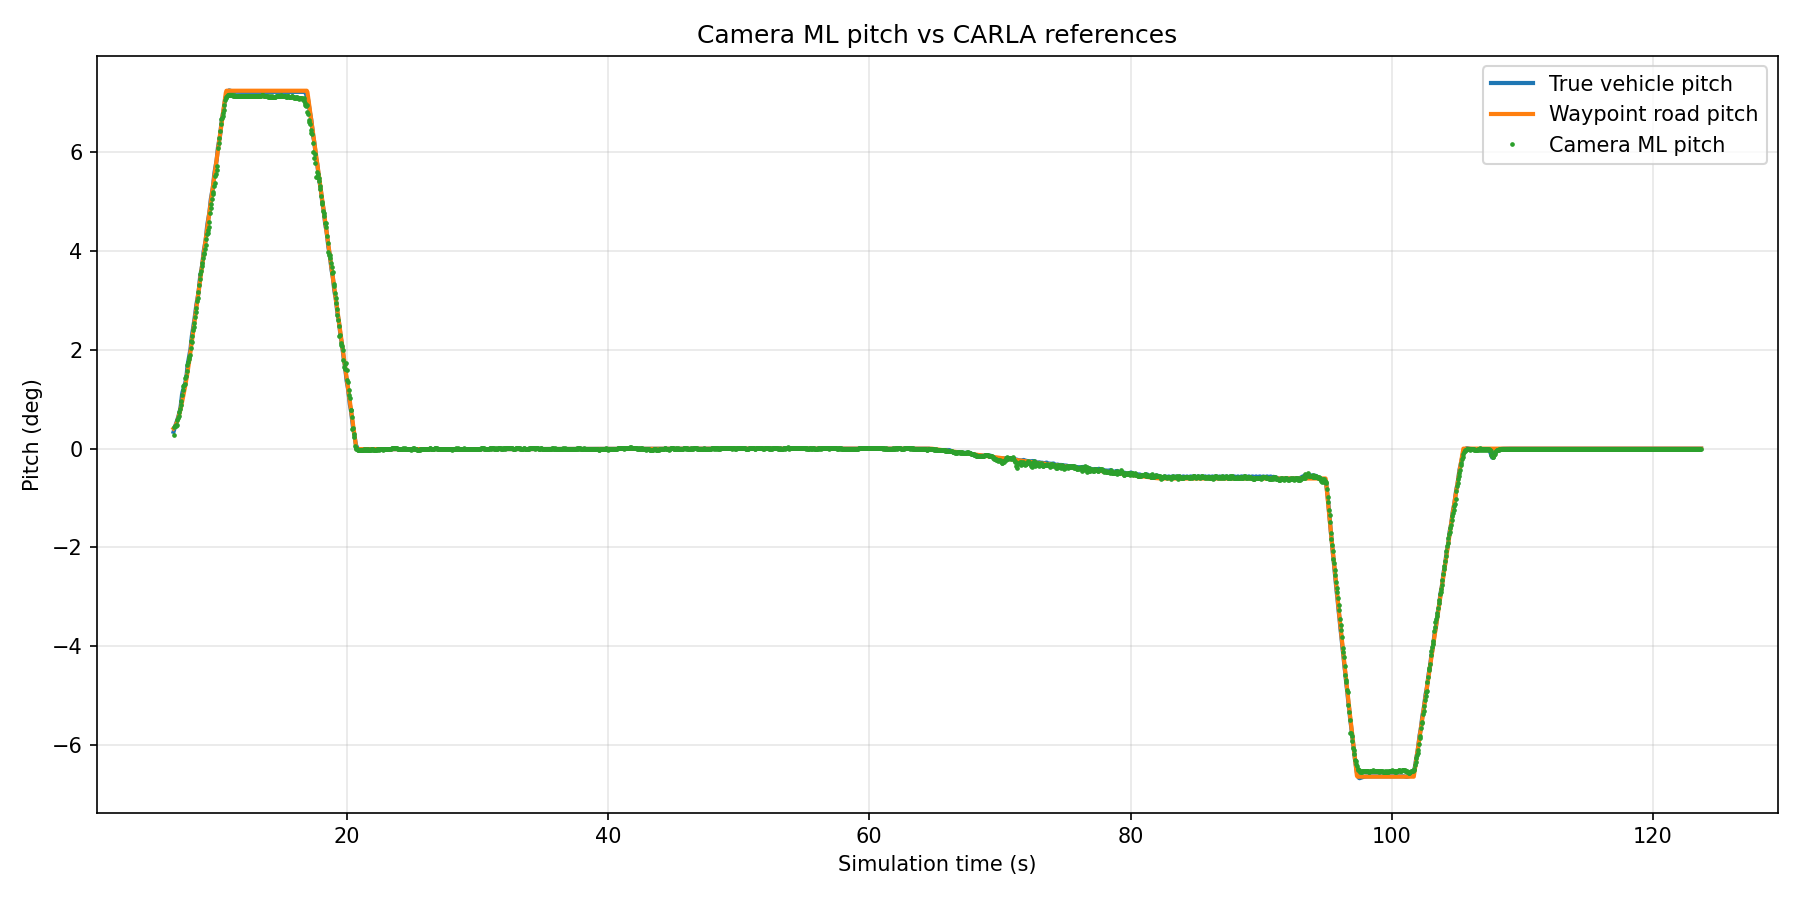
\includegraphics[width=\linewidth]{figures/camera_pitch_comparison.png}
    \caption{Camera-based pitch estimate compared with CARLA true vehicle pitch and waypoint road pitch.}
    \label{fig:camera_pitch}
\end{figure}

In the controlled simulation route, the semantic camera model closely follows both reference pitch signals. The use of road and road-line masks allows the model to rely on the geometric structure of the lane and road surface rather than unrelated visual content.

\subsection{GNSS Pitch Estimation Results}
Fig. \ref{fig:gnss_pitch} shows the GNSS-derived pitch estimate compared with the same CARLA references.

\begin{figure}[t]
    \centering
    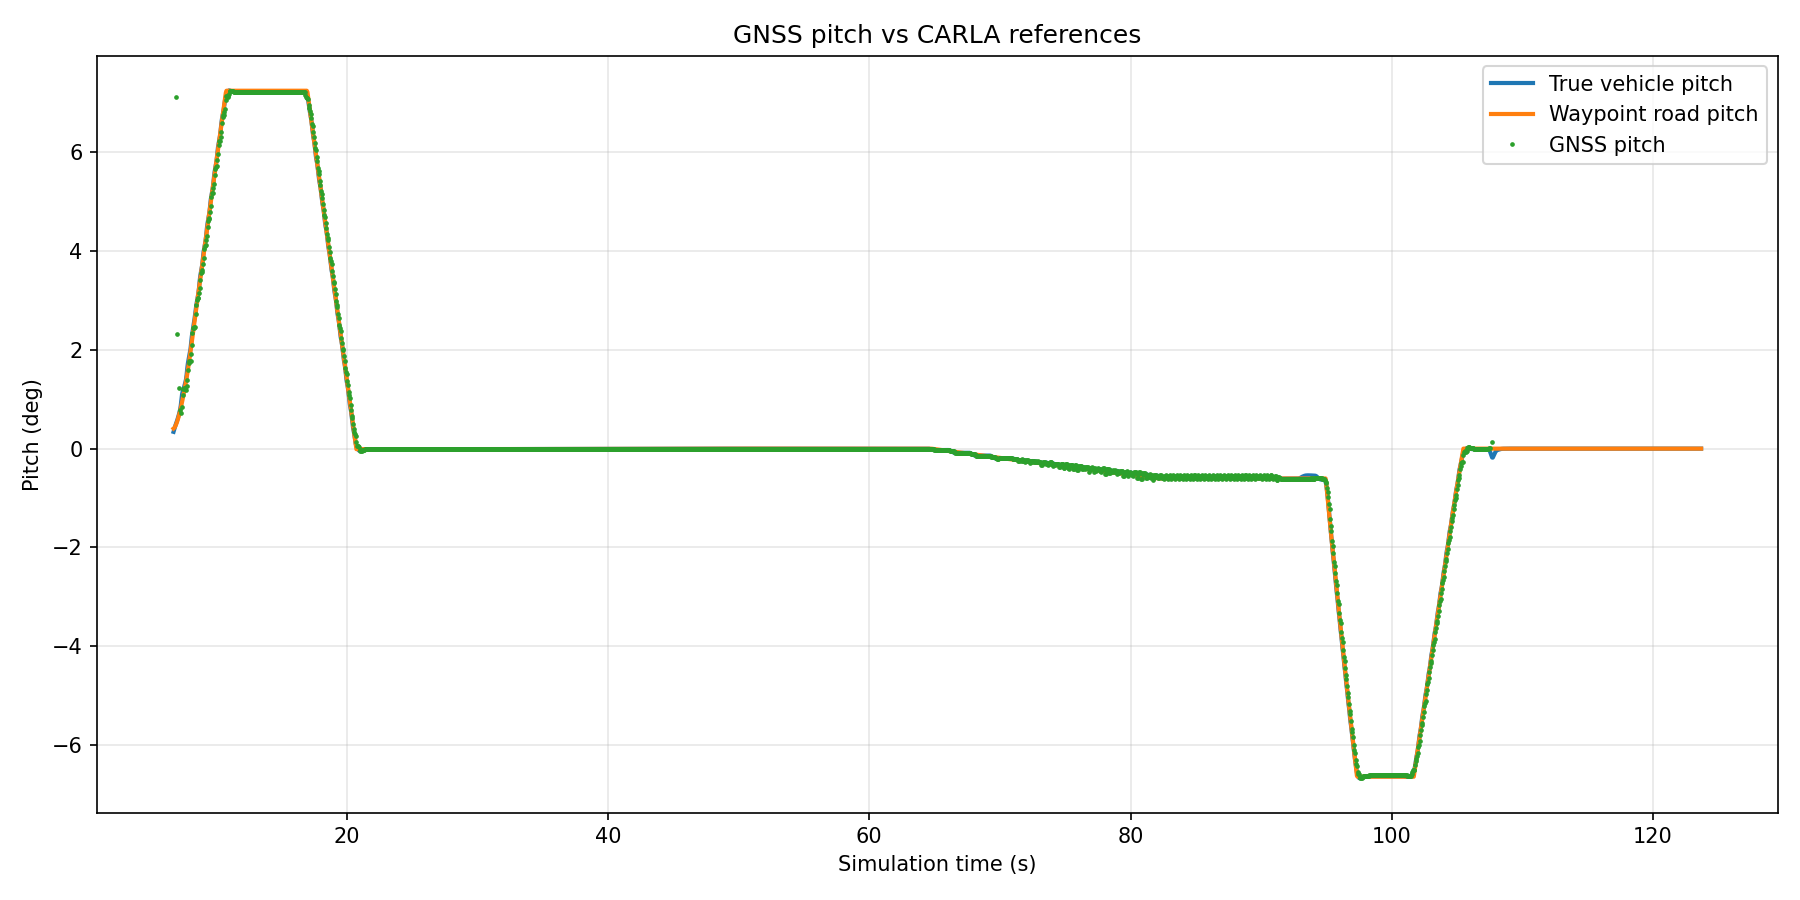
\includegraphics[width=\linewidth]{figures/gnss_pitch_comparison.png}
    \caption{GNSS-derived pitch estimate compared with CARLA reference pitch values.}
    \label{fig:gnss_pitch}
\end{figure}

The GNSS pitch estimate follows the general road-grade profile when sufficient movement is available. However, because it is computed from altitude change over horizontal displacement, it becomes sparse or unavailable when the vehicle is stationary. This demonstrates why GNSS-derived pitch was used as a baseline rather than the main filter correction measurement.

\subsection{Kalman Filter Fusion Results}
Fig. \ref{fig:kf_pitch} shows the final KF pitch estimate together with the camera measurement and CARLA references. The filter uses IMU gyroscope pitch rate for prediction and the camera ML pitch estimate for correction.

\begin{figure}[t]
    \centering
    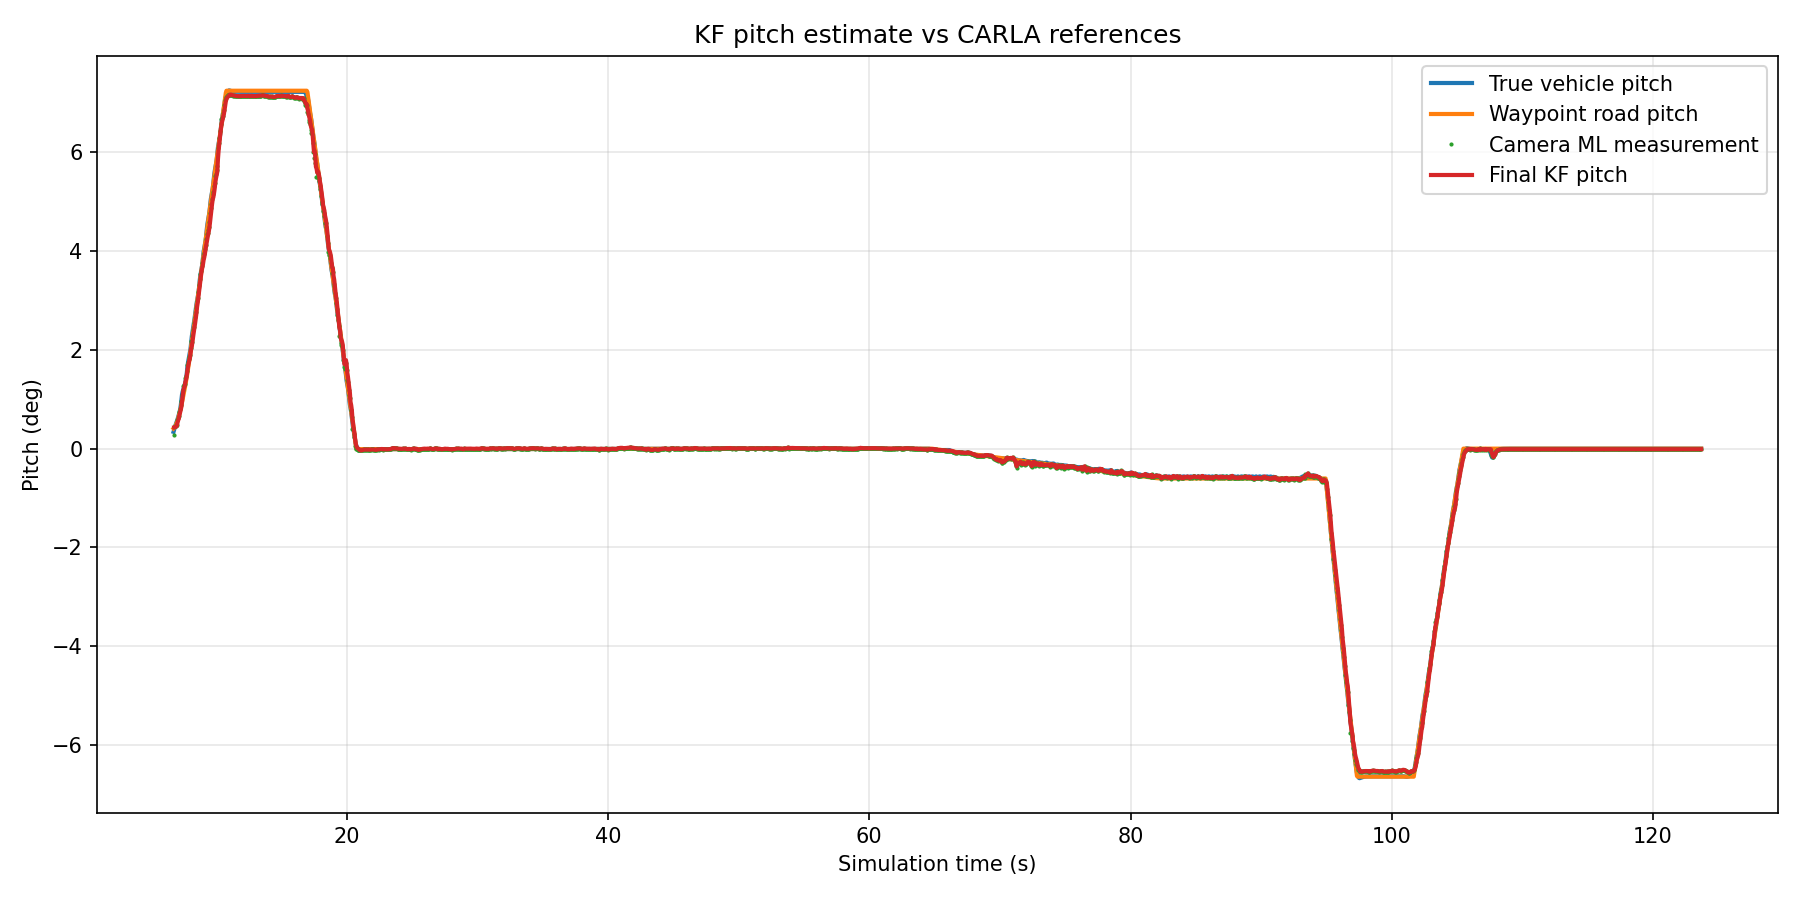
\includegraphics[width=\linewidth]{figures/kf_pitch_comparison.png}
    \caption{Final Kalman Filter pitch estimate compared with CARLA reference pitch values.}
    \label{fig:kf_pitch}
\end{figure}

The KF output follows the reference pitch profile closely while remaining consistent with the camera measurement. This behavior is expected because the camera measurement is accurate in the controlled route, while the IMU provides the short-term propagation between frames.

\subsection{Combined Sensor Comparison}
A combined comparison of the available pitch estimates is shown in Fig. \ref{fig:all_pitch}.

\begin{figure}[t]
    \centering
    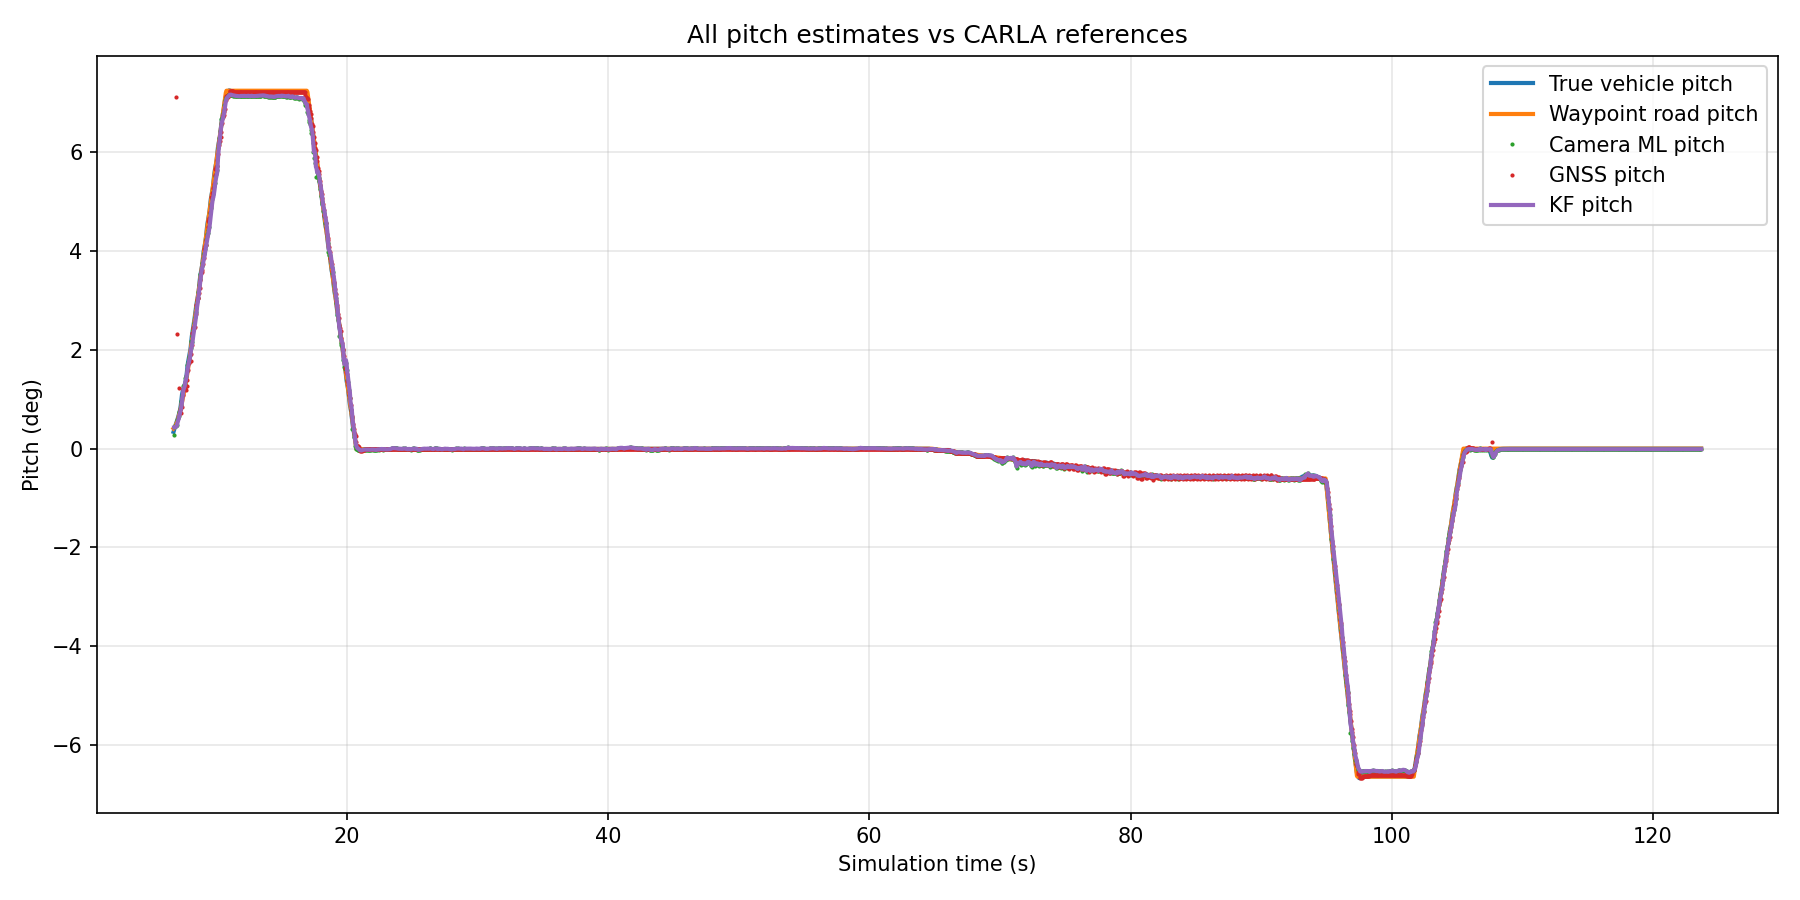
\includegraphics[width=\linewidth]{figures/all_sensors_pitch_comparison.png}
    \caption{Comparison of camera, GNSS, and KF pitch estimates with CARLA reference values.}
    \label{fig:all_pitch}
\end{figure}

The combined plot shows that the camera, GNSS, and KF estimates all follow the general slope profile during motion. However, the camera and KF estimates remain available at every camera frame, while the GNSS estimate depends on displacement between consecutive samples.

\subsection{Quantitative Error Summary}
Table \ref{tab:error_summary} summarizes the pitch estimation errors for the live CARLA run. The KF and camera estimates are evaluated over all available samples, while GNSS has fewer valid samples because it is not evaluated when horizontal displacement is below the threshold.

\begin{table}[t]
\caption{Pitch estimation error summary for the live CARLA run.}
\label{tab:error_summary}
\centering
\begin{tabular}{lccc}
\hline
Estimate & MAE (deg) & RMSE (deg) & Max (deg) \\
\hline
Camera vs true     & 0.028 & 0.050 & 0.408 \\
Camera vs waypoint & 0.032 & 0.057 & 0.465 \\
GNSS vs true       & 0.023 & 0.158 & 6.611 \\
GNSS vs waypoint   & 0.024 & 0.158 & 6.632 \\
KF vs true         & 0.034 & 0.063 & 0.366 \\
KF vs waypoint     & 0.035 & 0.062 & 0.349 \\
\hline
\end{tabular}
\end{table}


\section{Discussion}
The camera-based pitch estimator achieved the lowest error values in the evaluated route. However, the training and evaluation data were collected under controlled CARLA conditions using semantic road and road-line masks. Because the available road geometries, semantic classes, and environmental conditions are limited compared to real-world driving scenarios, the camera model benefits from a relatively constrained prediction problem.

In practical applications, camera measurements may be affected by unseen road geometries, occlusions, environmental changes, sensor noise, or temporary loss of visual features. Under such conditions, the IMU becomes increasingly important because it provides high-frequency motion information independent of visual scene content. The Kalman Filter framework therefore remains valuable even when the camera model is highly accurate, as it provides a mechanism for propagating pitch estimates between camera updates and improving robustness when camera measurements become degraded or unavailable.

\section{Conclusion}
This work presented a CARLA 0.9.16-based road pitch estimation pipeline using semantic camera measurements, IMU gyroscope input, GNSS baseline comparison, and Kalman Filter fusion. A MobileNet regression model was trained on semantic road and road-line masks to estimate pitch from road geometry. The camera model produced stable pitch estimates in the evaluated CARLA route and remained available even when GNSS-derived pitch was unavailable during stationary periods. Although the camera estimator achieved very low errors under the controlled simulation conditions, the Kalman Filter architecture provides a foundation for incorporating additional sensor information and improving robustness in more challenging environments. The final KF framework uses IMU gyroscope pitch rate for prediction and camera model output for measurement correction. The results demonstrate that the proposed simulation pipeline can estimate road pitch accurately under the tested CARLA route while keeping the system structure simple and interpretable.

\section{Acknowledgment}
The authors would like to thank Prof. Dr. Engin Masazade
for guidance and feedback during the project.\\

During the preparation of this manuscript, the authors used ChatGPT-5.5 solely for editing and grammatical enhancement to improve text readability. The authors reviewed all modifications and assume full responsibility for the final content.
\bibliographystyle{IEEEtran}
\bibliography{references}

\end{document}
